% vim: ts=4 sts=4 sw=4 et tw=75
\chapter{Notation}
\label{chap:notation}
\begin{quote}
    Perhaps of all the creations of man language is the most astonishing
    (惊讶的).
\end{quote}
\begin{quotesrc}
    Giles Lytton Strachey, \bookname{Words and Poetry}
\end{quotesrc}

The right language can make all the difference in how easy it is to write a
program. This is why a practicing programmer's arsenal holds not only
general-purpose languages like C and its relatives, but also programmable
shells, scripting languages, and lots of application-specific languages

The power of good notation reaches beyond traditional programming into
specialized problem domains. Regular expressions let us write compact (if
occasionally cryptic (神秘的)) definitions of classes of strings; HTML lets
us define the layout of interactive documents, often using embedded
programs in other languages such as JavaScript; Postscript expresses an
entire document -- this book, for example -- as a stylized program.
Spreadsheets and word processors often include programming languages like
Visual Basic to evaluate expressions, access information, or control
layout.

If you find yourself writing too much code to do a mundane (平凡的) job, or
if you have trouble expressing the process comfortably, maybe you're using
the wrong language. If the right language doesn't yet exist, that might be
an opportunity to create it yourself. Inventing a language doesn't
necessarily mean building the successor to Java; often a thorny (多刺的)
problem can be cleared up by a change of notation. Consider the format
strings in the \verb'printf' family, which are a compact and expressive way
to control the display of printed values.

In this chapter, we'll talk about how notation can solve problems, and
demonstrate some of the techniques you can use to implement your own
special-purpose languages. We'll even explore the possibilities of having
one program write another program, an apparently extreme use of notation
that happens more often, and is far easier to do, than many programmers
realize.

\section{Formatting Data}
\label{sec:formatting_data}

There is always a gap between what we want to say to the computer ("solve
my problem") and what we are required to say to get a job done. The
narrower this gap, the better. Good notation makes it easier to say what we
want and harder to say the wrong thing by mistake. Sometimes, good notation
can provide new insight (见识, 洞察), allowing us to solve problems that
seemed too difficult, or even lead us to new discoveries.

\term{Little languages} are specialized notations for narrow
domains. They not only provide a good interface but also help organize the
program that implements them. The \verb'printf' control sequences are a
good example:
\begin{wellcode}
    printf("%d %6.2f %-10.10s\n", i, f, s);
\end{wellcode}

Each \verb'%' in the format string signals a place to interpolate (插入)
the value of the next \verb'printf' argument; after some optional flags and
field widths, the terminating letter says what kind of parameter to expect.
This notation is compact, intuitive, and easy to write, and the
implementation is straightforward. The alternatives in C++
(\verb'iostream') and Java (\verb'java.io') seem more awkward (笨拙) since
they don't provide special notation, although they extend to user-defined
types and offer type-checking.

Some non-standard implementations of \verb'printf' let you add your own
conversions to the built-in set. This is convenient if you have other data
types that need output conversion. For example, a compiler might use
\verb'%L' for line number and file name; a graphics system might use
\verb'%P' for a point and \verb'%R' for a rectangle. The cryptic string of
letters and numbers for retrieving stock quotes (股价报价) that we saw in
Chapter \ref{chap:interface} was in the same spirit, a compact notation for
arranging (编排) combinations of stock data.

We can synthesize similar examples in C and C++. Suppose we want to send
packets containing various combinations of data types from one system to
another.  As we saw in Chapter \ref{chap:portability}, the cleanest
solution may be to convert to a textual representation. For a standard
network protocol, though, the format is likely to be binary for reasons of
efficiency or size. How can we write the packet-handling code to be
portable, efficient, and easy to use?

To make this discussion concrete, imagine that we plan to send packets of
8-bit, 16-bit, and 32-bit data items from system to system. ANSI C says
that we can always store at least 8 bits in a \verb'char', 16 bits in a
\verb'short', and 32 bits in a \verb'long', so we will use these data types
to represent our values. There will be many types of packets; packet type 1
might have a 1-byte type specifier, a 2-byte count, a 1-byte value and a
4-byte data item:
\begin{center}
    \begin{tikzpicture}
        \pgfmathsetmacro\width{1.5};

        \draw (0, 0) -- (\width * 8, 0);
        \draw (0, 1) -- (\width * 8, 1);
        \foreach \i in {0, ..., 8}
        \draw (\i * \width, 0) -- (\i * \width, 1);

        \newcounter{j};
        \setcounter{j}{0};
        \foreach \ind/\data in { 0/\texttt{0x01}, 1/\texttt{cnt$_1$},
            2/\texttt{cnt$_0$}, 3/\texttt{val}, 4/\texttt{data$_3$},
            5/\texttt{data$_2$}, 6/\texttt{data$_1$},
            7/\texttt{data$_0$}} {

            \node at (\arabic{j} * \width + \width / 2, 0.5)
                {\data};
            \addtocounter{j}{1};
        }
    \end{tikzpicture}
\end{center}
Packet type 2 might contain a short and two long data words:
\begin{center}
    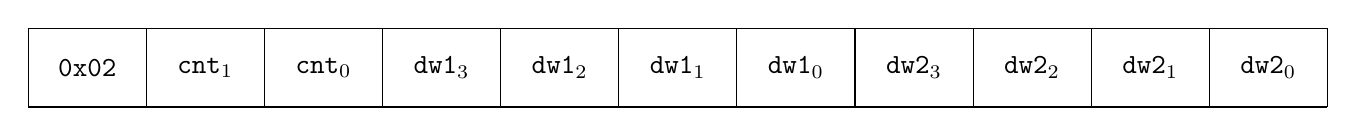
\begin{tikzpicture}
        \pgfmathsetmacro\width{1.5};

        \draw (0, 0) -- (\width * 11, 0);
        \draw (0, 1) -- (\width * 11, 1);
        \foreach \i in {0, ..., 11}
        \draw (\i * \width, 0) -- (\i * \width, 1);

        \setcounter{j}{0};
        \foreach \ind/\data in { 0/\texttt{0x02}, 1/\texttt{cnt$_1$},
            2/\texttt{cnt$_0$}, 3/\texttt{dw1$_3$},
            4/\texttt{dw1$_2$}, 5/\texttt{dw1$_1$},
            6/\texttt{dw1$_0$}, 7/\texttt{dw2$_3$}, 8/\texttt{dw2$_2$},
            9/\texttt{dw2$_1$}, 10/\texttt{dw2$_0$}} {

            \node at (\arabic{j} * \width + \width / 2, 0.5)
                {\data};
            \addtocounter{j}{1};
        }
    \end{tikzpicture}
\end{center}

One approach is to write pack and unpack functions for each possible packet
type:
\begin{wellcode}
    int pack_type1(unsigned char *buf, unsigned short count,
            unsigned char val, unsigned long data)
    {
        unsigned char *bp;

        bp = buf;
        *bp++ = 0x01;
        *bp++ = count >> 8;
        *bp++ = count;
        *bp++ = val;
        *bp++ = data >> 24;
        *bp++ = data >> 16;
        *bp++ = data >> 8;
        *bp++ = data;
        return bp - buf;
    }
\end{wellcode}
For a realistic protocol, there will be dozens of such routines, all
variations on a theme. The routines could be simplified by using macros or
functions to handle the basic data types (\verb'short', \verb'long', and so
on), but even so, such repetitive code is easy to get wrong, hard to read,
and hard to maintain.

The inherent (固有的) repetitiveness (重复性) of the code is a clue that
notation can help.  Borrowing the idea from \verb'printf', we can define a
tiny specification language in which each packet is described by a brief
string that captures the packet layout.  Successive elements of the packet
are encoded with \verb'c' for an 8-bit character, \verb's' for a 16-bit
short integer, and \verb'l' for a 32-bit long integer. Thus, for example,
the packet type 1 built by our example above, including the initial type
byte, might be described by the format string \verb'cscl'. Then we can use
a single pack function to create packets of any type; this packet would be
created with
\begin{wellcode}
    pack(buf, "cscl", 0x01, count, val, data);
\end{wellcode}
Because our format string contains only data definitions, there's no need
for the \verb'%' character used by \verb'printf'.

In practice, information at the beginning of the packet might tell the
recipient (接受者) how to decode the rest, but we'll assume the first byte
of the packet can be used to determine the layout. The sender encodes the
data in this format and ships it; the receiver reads the packet, picks off
the first byte, and uses that to decode what follows.

Here is an implementation of \verb'pack', which fills \verb'buf' with the
encoded representation of its arguments as determined by the format. We
make all values unsigned, including the bytes in the packet buffer, to
avoid sign-extension problems.  We also use some conventional
\verb'typedef's to keep the declarations short:
\begin{wellcode}
    typedef unsigned char   uchar;
    typedef unsigned short  ushort;
    typedef unsigned long   ulong;
\end{wellcode}
Like \verb'sprintf', \verb'strcpy', and similar functions, \verb'pack'
assumes that the buffer is big enough to hold the result; it is the
caller's responsibility to ensure this. There is also no attempt to detect
mismatches between the format and the argument list.
\begin{wellcode}
    #include <stdarg.h>

    /* pack: pack binary items into buf, return length */
    int pack(uchar *buf, char *fmt, ...)
    {
        va_list args;
        char    *p;
        uchar   *bp;
        ushort  s;
        ulong   l;
        bp = buf;
        va_start(args, fmt);
        for (p = fmt; *p != '\0'; p++) {
            switch (*p) {
            case 'c':   /* char */
                *bp++ = va_arg(args, int);
                break;
            case 's':   /* short */
                s = va_arg(args, int);
                *bp++ = s >> 8;
                *bp++ = s;
                break;
            case 'l':   /* long */
                l = va_arg(args, ulong);
                *bp++ = l >> 24;
                *bp++ = l >> 16;
                *bp++ = l >> 8;
                *bp++ = l;
                break;
            default:    /* illegal type character */
                va_end(args);
                return -1;
            }
        }
        va_end(args);
        return bp - buf;
    }
\end{wellcode}

The \verb'pack' routine uses the \verb'stdarg.h' header more extensively
than \verb'eprintf' did in Chapter \ref{chap:interface}. The successive
arguments are extracted using the macro \verb'va_arg', with first operand
the variable of type \verb'va_list' set up by calling \verb'va_start' and
second operand the type of the argument (this is why \verb'va_arg' is a
macro, not a function).  When processing is done, \verb'va_end' must be
called. Although the arguments for \verb"'c'" and \verb"'s'" represent
\verb'char' and \verb'short' values, they must be extracted as \verb'int's
because C promotes (提升) \verb'char' and \verb'short' arguments to
\verb'int' when they are represented by an ellipsis \verb'...'  parameter.

Each \verb'pack_type' routine will now be one line long, marshaling
(封装处理) its arguments into a call of \verb'pack':
\begin{wellcode}
    /* pack_type1: pack format 1 packet */
    int pack_type1(uchar *buf, ushort count, uchar val, ulong data)
    {
        return pack(buf, "cscl", 0x01, count, val, data);
    }
\end{wellcode}

To unpack, we can do the same thing: rather than write separate code to
crack each packet format, we call a single \verb'unpack' with a format
string. This centralizes the conversion in one place:
\begin{wellcode}
    /* unpack: unpack packed items from buf, return length */
    int unpack(uchar *buf, char *fmt, ...)
    {
        va_list args;
        char    *p;
        uchar   *bp, *pc;
        ushort  *ps;
        ulong   *pl;

        bp = buf;
        va_start(args, fmt);
        for (p = fmt; *p != '\0'; p++) {
            switch (*p) {
            case 'c':   /* char */
                pc = va_arg(args, uchar *);
                *pc = *bp++;
                break;
            case 's':   /* short */
                ps = va_arg(args, ushort *);
                *ps = *bp++ << 8;
                *ps |= *bp++;
                break;
            case 'l':   /* long */
                pl = va_arg(args, ulong *);
                *pl = *bp++ << 24;
                *pl |= *bp++ << 16;
                *pl |= *bp++ << 8;
                *pl |= *bp++;
                break;
            default:    /* illegal type character */
                va_end(args);
                return -1;
            }
        }
        va_end(args);
        return bp - buf;
    }
\end{wellcode}
Like \verb'scanf', \verb'unpack' must return multiple values to its caller,
so its arguments are pointers to the variables where the results are to be
stored. Its function value is the number of bytes in the packet, which can
be used for error checking.

Because the values are unsigned and because we stayed within the sizes that
ANSI C defines for the data types, this code transfers data portably even
between machines with different sizes for \verb'short' and \verb'long'.
Provided (倘若) the program that uses \verb'pack' does not try to send as a
long (for example) a value that cannot be represented in 32 bits, the value
will be received correctly. In effect, we transfer the low 32 bits of the
value.  If we need to send larger values, we could define another format.

The type-specific unpacking routines that call \verb'unpack' are easy:
\begin{wellcode}
    /* unpack_type2: unpack and process type 2 packet */
    int unpack_type2(int n, uchar *buf)
    {
        uchar   c;
        ushort  count;
        ulong   dw1, dw2;

        if (unpack(buf, "csll", &c, &count, &dw1, &dw2) != n)
            return -1;
        assert(c == 0x02);
        return process_type2(count, dw1, dw2);
    }
\end{wellcode}
To call \verb'unpack_type2', we must first recognize that we have a type 2
packet, which implies a receiver loop something like this:
\begin{wellcode}
    while ((n = readpacket(network, buf, BUFSIZ)) > 0) {
        switch (buf[0]) {
        default:
            eprintf("bad packet type 0x%x", buf[0]);
            break;
        case 1:
            unpack_type1(n, buf);
            break;
        case 2:
            unpack_type2(n, buf);
            break:
        ...
        }
    }
\end{wellcode}
This style of programming can get long-winded (冗长的). A more compact
method is to define a table of function pointers whose entries are the
unpacking routines indexed by type:
\begin{wellcode}
    int (*unpackfn[])(int, uchar *) = {
        unpack_type0,
        unpack_type1,
        unpack_type2,
    };
\end{wellcode}
Each function in the table parses a packet, checks the result, and
initiates further processing for that packet. The table makes the
recipient's job straightforward:
\begin{wellcode}
    /* receive: read packets from network, process them */
    void receive(int network)
    {
        uchar   type, buf[BUFSIZ];
        int     n;

        while ((n = readpacket(network, buf, BUFSIZ)) > 0) {
            type = buf[0];
            if (type >= NELEMS(unpackfn))
                eprintf("bad packet type 0x%x", type);
            if ((*unpackfn[type](n, buf) < 0)
                eprintf("protocol error, type %x length %d",
                        type, n);
        }
    }
\end{wellcode}
Each packet's handling code is compact, in a single place, and easy to
maintain. The receiver is largely independent of the protocol itself; it's
clean and fast, too.

This example is based on some real code for a commercial networking
protocol.  Once the author realized this approach could work, a few
thousand repetitive, error-prone (容易出错的) lines of code shrunk (压缩)
to a few hundred lines that are easily maintained. Notation reduced the
mess enormously.

\begin{exercise}
    Modify \verb'pack' and \verb'unpack' to transmit signed values
    correctly, even between machines with different sizes for \verb'short'
    and \verb'long'. How should you modify the format strings to specify a
    signed data item? How can you test the code to check, for example, that
    it correctly transfers a \verb'-1' from a computer with 32-bit
    \verb'long's to one with 64-bit \verb'long's?
\end{exercise}
\begin{exercise}
    Extend \verb'pack' and \verb'unpack' to handle strings; one possibility
    is to include the length of the string in the format string. Extend
    them to handle repeated items with a count. How does this interact with
    the encoding of strings?
\end{exercise}
\begin{exercise}
    The table of function pointers in the C program above is at the heart
    of C++'s virtual function mechanism. Rewrite \verb'pack' and
    \verb'unpack' and receive in C++ to take advantage of this notational
    convenience.
\end{exercise}
\begin{exercise}
    Write a command-line version of \verb'printf' that prints its second
    and subsequent arguments in the format given by its first argument.
    Some shells already provide this as a built-in.
\end{exercise}
\begin{exercise}
    Write a function that implements the format specifications found in
    spreadsheet programs or in Java's \verb'DecimalFormat' class, which
    display numbers according to patterns that indicate mandatory and
    optional digits, location of decimal points and commas, and so on. To
    illustrate, the format
    \begin{wellcode}
        ##,##0.00
    \end{wellcode}
    specifies a number with two decimal places, at least one digit to the
    left of the decimal point, a comma after the thousands digit, and
    blank-filling up to the ten-thousands It would represent
    \verb'12345.67' as \verb'12,345.67' and \verb'.4' as
    \texttt{\textvisiblespace\textvisiblespace
        \textvisiblespace\textvisiblespace0.4} (using \textvisiblespace 
    \ to stand for blanks). For a full specification, look at the definition
    of \verb'DecimalFormat' or a spreadsheet program.
\end{exercise}

\section{Regular Expressions}
\label{sec:regular_expressions}

The format specifiers (说明) for \verb'pack' and \verb'unpack' are a very
simple notation for defining the layout of packets. Our next topic is a
slightly more complicated but much more expressive notation,
\term{regular expressions}, which specify patterns of text.
We've used regular expressions occasionally throughout the book without
defining them precisely; they are familiar enough to be understood without
much explanation.  Although regular expressions are pervasive (无孔不入的)
in the Unix programming environment, they are not as widely used in other
systems, so in this section we'll demonstrate some of their power. In case
you don't have a regular expression library handy, we'll also show a
rudimentary (低级的) implementation.

There are several flavors (滋味) of regular expressions, but in spirit they
are all the same, a way to describe patterns of literal characters, along
with repetitions, alternatives, and shorthands (简写) for classes of
characters like digits or letters. One familiar example is the so-called
"wildcards" used in command-line processors or shells to match patterns of
file names. Typically a is taken to mean "any string of characters" so, for
example, a command like
\begin{wellcode}
    C:\>del *.exe
\end{wellcode}
uses a pattern that matches all files whose names consist of any string
ending in \verb'".exe"'. As in often the case, details differ from system
to system, and even from program to program.

Although the vagaries (奇特行为) of different programs may suggest that
regular expressions are an ad hoc (特别设的) mechanism, in fact they are a
language with a formal grammar and a precise meaning for each utterance
(言辞) in the language. Furthermore, the right implementation can run very
fast; a combination of theory and engineering practice makes a lot of
difference (造成了很多差异), an example of the benefit of specialized
algorithms that we alluded (提及) to in Chapter \ref{chap:alds}.

A regular expression is a sequence of characters that defines a set of
matching strings. Most characters simply match themselves, so the regular
expression \verb'abc' will match that string of letters wherever it occurs.
In addition a few metacharacters indicate repetition or grouping or
positioning. In conventional Unix regular expressions, \verb'^' stands for
the beginning of a string and \verb'$' for the end, so \verb'^x' matches an
\verb'x' only at the beginning of a string. \verb'x$' matches an \verb'x'
only at the end, \verb'^x$' matches \verb'x' only if it is the sole
(仅有的) character of the string, and \verb'^$' matches the empty string.

The character "\verb'.'" matches any character, so \verb'x.y' matches
\verb'xay', \verb'x2y' and so on, but not \verb'xy' or \verb'xaby', and
\verb'^.$' matches a string with a single arbitrary character.

A set of characters inside brackets \verb'[]' matches any one of the
enclosed characters, so \verb'[0123456789]' matches a single digit; it may
be abbreviated \verb'[0-9]'.

These building blocks are combined with parentheses for grouping, \verb'|'
for alternatives, \verb'*' for zero or more occurrences, \verb'+' for one or
more occurrences, and \verb'?' for zero or one occurrences. Finally, \verb'\'
is used as a prefix to quote a metacharacter and turn off its special
meaning; \verb'\*' is a literal \verb'*' and \verb'\\' is a literal
backslash.

The best-known regular expression tool is the program \verb'grep' that
we've mentioned several times. The program is a marvelous (了不起的)
example of the value of notation.  It applies a regular expression to each
line of its input files and prints those lines that contain matching
strings. This simple specification, plus the power of regular expressions,
lets it solve many day-to-day (日复一日) tasks. In the following examples,
note that the regular expression syntax used in the argument to \verb'grep'
is different from the wildcards used to specify a set of file names; this
difference reflects the different uses.

Which source file uses class \verb'Regexp'?
\begin{wellcode}
    % grep Regexp *.java
\end{wellcode}

Which implements it?
\begin{wellcode}
    % grep 'class.*Regexp' *.java
\end{wellcode}

Where did I save that mail from Bob?
\begin{wellcode}
    grep '^From:.* bob@' mail/*
\end{wellcode}

How many non-blank source lines are there in this program?
\begin{wellcode}
    % grep '.' *.cpp | wc
\end{wellcode}

With flags to print line numbers of matched lines, count matches, do case-
insensitive matching, invert the sense (select lines that don't match the
pattern), and perform other variations of the basic idea, \verb'grep' is so
widely used that it has become the classic example of tool-based
programming.

Unfortunately, not every system comes with \verb'grep' or an equivalent.
Some systems include a regular expression library, usually called
\verb'regex' or \verb'regexp', that you can use to write a version of
\verb'grep'. If neither option is available, it's easy to implement a
modest (适度的) subset of the full regular expression language. Here we
present an implementation of regular expressions, and \verb'grep' to go
along with it; for simplicity, the only metacharacters are \verb'^ $'. and
\verb'*', with \verb'*' specifying a repetition of the single previous
period (片段) or literal character. This subset provides a large fraction
of the power with a tiny fraction of the programming complexity of general
expressions.

Let's start with the \verb'match' function itself, Its job is to determine
whether a text string matches a regular expression:
\begin{wellcode}
    /* match: search for regexp anywhere in text */
    int match(char *regexp, char *text)
    {
        if (regexp[0] == '^')
            return matchhere(regexp+1, text);
        do {    /* must look even if string is empty */
            if (matchhere(regexp, text))
                return 1;
        } while (*text++ != '\0');
        return 0;
    }
\end{wellcode}
If the regular expression begins with \verb'^', the text must begin with a
match of the remainder of the expression. Otherwise, we walk along the
text, using \verb'matchhere' to see if the text matches at any position. As
soon as we find a match, we're done. Note the use of a \verb'do-while':
expressions can match the empty string (for example, \verb'$' matches the
empty string at the end of a line and \verb'.*' matches any number of
characters, including zero), so we must call matchhere even if the text is
empty.

The recursive function \verb'matchhere' does most of the work:
\begin{wellcode}
    /* matchhere: search for regexp at beginning of text */
    int matchhere(char *regexp, char *text)
    {
        if (regexp[0] == '\0')
            return 1;
        if (regexp[1] == '*')
            return matchstar(regexp[0], regexp+2, text);
        if (regexp[0] == '$' && regexp[1] == '\0')
            return *text == '\0';
        if (*text != '\0' && (regexp[0] == '.' || regexp[0] == *text))
            return matchhere(regexp+1, text+1);
        return 0;
    }
\end{wellcode}
If the regular expression is empty, we have reached the end and thus have
found a match. If the expression ends with \verb'$', it matches only if the
text is also at the end. If the expression begins with a period, that
matches any character. Otherwise the expression begins with a plain
character that matches itself in the text. A \verb'^' or \verb'$' that
appears in the middle of a regular expression is thus taken as a literal
character, not a metacharacter.

Notice that matchhere calls itself after matching one character of pattern
and string, so the depth of recursion can be as much as the length of the
pattern.

The one tricky case occurs when the expression begins with a starred
character, for example \verb'x*'. Then we call \verb'matchstar', with first
argument the operand of the star (\verb'x') and subsequent arguments the
pattern after the star and the text.
\begin{wellcode}
    /* matchstar: search for c*regexp at beginning of text */
    int matchstar(int c, char *regexp, char *text)
    {
        do {    /* a * matches zero or more instances */
            if (matchhere(regexp, text))
                return 1;
        } while (*text != '\0' && (*text++ == c || c == '.'));
        return 0;
    }
\end{wellcode}
Here is another \verb'do-while', again triggered by the requirement that
the regular expression \verb'x*' can match zero characters. The loop checks
whether the text matches the remaining expression, trying at each position
of the text as long as the first character matches the operand of the star.

This is an admittedly (诚然地) unsophisticated implementation, but it
works, and at fewer than 30 lines of code, it shows that regular
expressions don't need advanced techniques to be put to use.

We'll soon present some ideas for extending the code. For now, though,
let's write a version of \verb'grep' that uses \verb'match'. Here is the
main routine:
\begin{wellcode}
    /* grep main: search for regexp in files */
    int main(int argc, char *argv[])
    {
        int     i, nmatch;
        FILE    *f;

        setprogname("grep");
        if (argc < 2)
            eprintf("usage: grep regexp [file ...]");
        nmatch = 0;
        if (argc == 2) {
            if (grep(argv[1], stdin, NULL))
                nmatch++;
        } else {
            for (i = 2; i < argc; i++) {
                f = fopen(argv[i], "r");
                if (f == NULL) {
                    weprintf("can't open %s:", argv[i]);
                    continue;
                }
                if (grep(argv[1], f, argc > 3 ? argv[i] : NULL) > 0)
                    nmatch++;
                fclose(f);
            }
        }
        return nmatch == 0;
    }
\end{wellcode}
It is conventional that C programs return 0 for success and non-zero values
for various failures. Our \verb'grep', like the Unix version, defines
success as finding a matching line, so it returns \verb'0' if there were
any matches, \verb'1' if there were none, and \verb'2' (via \verb'eprintf')
if an error occurred. These status values can be tested by other programs
like a shell.

The function \verb'grep' scans a single file, calling
\verb'match' on each line:
\begin{wellcode}
    /* grep: search for regexp in file */
    int grep(char *regexp, FILE *f, char *name)
    {
        int     n, nmatch;
        char    buf[BUFSIZ];

        nmatch = 0;
        while (fgets(buf, sizeof(buf), f) != NULL) {
            n = strlen(buf);
            if (n > 0 && buf[n-1] == '\n')
                buf[n-1] = '\0';
            if (match(regexp, buf)) {
                nmatch++;
                if (name != NULL)
                    printf("%s: ", name);
                printf("%s\n", buf);
            }
        }
        return nmatch;
    }
\end{wellcode}

The main routine doesn't quit if it fails to open a file. This design was
chose because it's common to say something like
\begin{wellcode}
    % grep herpolhode *.*
\end{wellcode}
and find that one of the files in the directory can't be read. It's better
for \verb'grep' to keep going after reporting the problem, rather than to
give up and force the user to type the file list manually to avoid the
problem file. Also, notice that \verb'grep' prints the file name and the
matching line, but suppresses the name if it is reading standard input or a
single file. This may seem an odd (古怪的) design, but it reflects an
idiomatic style of use based on experience. When given only one input,
\verb'grep''s task is usually selection, and the file name would clutter
(弄乱) the output. But if it is asked to search through many files, the
task is most often to find all occurrences of something, and the names are
informative. Compare
\begin{wellcode}
    % strings markov.exe | grep 'DOS mode'
\end{wellcode}
with
\begin{wellcode}
    % grep grammer chapter*.txt
\end{wellcode}
These touches are part of what makes \verb'grep' so popular, and
demonstrate that notation must be packaged with human engineering to build
a natural, effective tool.

Our implementation of \verb'match' returns as soon as it finds a match. For
\verb'grep', that is a fine default. But for implementing a substitution
(search-and-replace) operator in a text editor the \term{leftmost longest}
match is more suitable. For example, given the text
\verb'"aaaaa"' the pattern \verb'a*' matches the null string at the
beginning of the text, but it seems more natural to match all five
\verb'a''s. To cause \verb'match' to find the leftmost longest string,
\verb'matchstar' must be rewritten to be greedy: rather than looking at
each character of the text from left to right, it should skip over the
longest string that matches the starred operand, then back up (倒退) if the
rest of the string doesn't match the rest of the pattern. In other words,
it should run from right to left. Here is a version of \verb'matchstar'
that does leftmost longest matching:
\begin{wellcode}
    /* matchstar: leftmost longest search for c*regexp */
    int matchstar(int c, char *regexp, char *text)
    {
        char    *t;

        for (t = text; *t != '\0' && (*t == c || c == '.');
                t++)
            ;
        do {    /* matches zero or more */
            if (matchhere(regexp, t))
                return 1;
        } while (t-- > text);
        return 0;
    }
\end{wellcode}
It doesn't matter which match \verb'grep' finds, since it is just checking
for the presence of any match and printing the whole line. So since
leftmost longest matching does extra work, it's not necessary for
\verb'grep', but for a substitution operator, it is essential.

Our \verb'grep' is competitive with system-supplied versions, regardless of
the regular expression. There are pathological (错误的) expressions that
can cause exponential behavior, such as \verb'a*a*a*a*a*b' when given the
input \verb'aaaaaaaaac', but the exponential behavior is present in some
commercial implementations too. A \verb'grep' variant available on Unix,
called \verb'egrep', uses a more sophisticated matching algorithm that
guarantees linear performance by avoiding backtracking when a partial match
fails.

What about making \verb'match' handle full regular expressions? These would
include character classes like \verb'[a-zA-Z]' to match an alphabetic
character, the ability to quote a metacharacter (for example to search for
a literal period), parentheses for grouping, and alternatives (\verb'abc'
or \verb'def'). The first step is to help \verb'match' by compiling the
pattern into a representation that is easier to scan. It is expensive to
parse a character class every time we compare it against a character; a
pre-computed representation based on bit vectors could make character
classes much more efficient. For full regular expressions, with parentheses
and alternatives, the implementation must be more sophisticated, but can
use some of the techniques we'll talk about later in this chapter.

\begin{exercise}
    How does the performance of \verb'match' compare to \verb'strstr' when
    searching for plain text?
\end{exercise}

\begin{exercise}
    Write a non-recursive version of \verb'matchhere' and compare its
    performance to the recursive version.
\end{exercise}

\begin{exercise}
    Add some options to \verb'grep'. Popular ones include \verb'-v' to
    invert the sense of the \verb'match'. \verb'-i' to do case-insensitive
    matching of alphabetics, and \verb'-n' to include line numbers in the
    output. How should the line numbers be printed? Should they be printed
    on the same line as the matching text?
\end{exercise}

\begin{exercise}
    Add the \verb'+' (one or more) and \verb'?' (zero or one) operators to
    \verb'match'. The pattern \verb'a+bb?' matches one or more \verb'a''s
    followed by one or two \verb'b''s.
\end{exercise}

\begin{exercise}
    The current implementation of match turns off the special meaning of
    \verb'^' and \verb'$' if they don't begin or end the expression, and of
    \verb'*' if it doesn't immediately follow a literal character or a
    period. A more conventional design is to quote a metacharacter by
    preceding it with a backslash. Fix \verb'match' to handle backslashes
    this way.
\end{exercise}

\begin{exercise}
    Add character classes to \verb'match'. Character classes specify a
    match for any one of the characters in the brackets. They can be made
    more convenient by adding ranges, for example \verb'[a-z]' to match any
    lower-case letter, and inverting the sense, for example \verb'[^O-9]'
    to match any character except a digit.
\end{exercise}

\begin{exercise}
    Change \verb'match' to use the leftmost-longest version of
    \verb'matchstar', and modify it to return the character positions of
    the beginning and end of the matched text. Use that to build a program
    \verb'gres' that is like \verb'grep' but prints every input line after
    substituting new text for text that matches the pattern, as in
    \begin{wellcode}
        % grep 'homoiousian' 'homoousian' mission.stmt
    \end{wellcode}
\end{exercise}

\begin{exercise}
    Modify \verb'match' and \verb'grep' to work with UTF-8 strings of
    Unicode characters. Because UTF-8 and Unicode are a superset of ASCII,
    this change is upwardly compatible. Regular expressions, as well as the
    searched text, will also need to work properly with UTF-8. How should
    character classes be implemented?
\end{exercise}

\begin{exercise}
    Write an automatic tester for regular expressions that generates test
    expressions and test strings to search. If you can, use an existing
    library as a reference implementation; perhaps you will find bugs in it
    too.
\end{exercise}

\section{Programmable Tools}
\label{sec:programmable_tools}

Many tools are structured around a special-purpose language. The
\verb'grep' program is just one of a family of tools that use regular
expressions or other languages to solve programming problems.

One of the first examples was the command interpreter or job control
language. It was realized early that common sequences of commands could be
placed in a file, and an instance of the command interpreter or
\textit{shell} could be executed with that file as input. From there it was
a short step to adding parameters, conditionals, loops, variables, and all
the other trappings of a conventional programming language.  The main
difference was that there was only one data type -- strings -- and the
operators in shell programs tended to be entire programs that did
interesting computations.  Although shell programming has fallen out of
favor (失宠), often giving ground to alternatives like Perl in command
environments and to pushing buttons in graphical user interfaces, it is
still an effective way to build up complex operations out of simpler
pieces.

Awk is another programmable tool, a small, specialized pattern-action
language that focuses on selection and transformation of an input stream.
As we saw in Chapter \ref{chap:desipl}, Awk automatically reads input files
and splits each line into fields called \verb'$1' through \verb'$NF', where
\verb'NF' is the number of fields on the line. By providing default
behavior for many common tasks, it makes useful one-line programs possible.
For example, this complete Awk program,
\begin{wellcode}
    # split.awk: split input into one word per line
    { for (i = 1; i <= NF; i++) print $i }
\end{wellcode}
prints the "words" of each input line one word per line. To go in the other
direction, here is an implementation of \verb'fmt', which fills each output
line with words, up to at most 60 characters; a blank line causes a
paragraph break.
\begin{wellcode}
    # fmt.awk: format into 60-character lines
    /./  { for (i = 1; i <= NF; i++) addword($i) }  # non-blank line
    /^$/ { printline(); print "" }                  # blank line
    END  { printline() }

    function addword(w) {
        if (length(line) + 1 + length(w) > 60)
            printline()
        if (length(line) == 0)
            line = w
        else
            line = line " " w
    }

    function printline() {
        if (length(line) > 0) {
            print line
            line = ""
        }
    }
\end{wellcode}
We often use \verb'fmt' to re-paragraph mail messages and other short
documents; we also use it to format the output of Chapter
\ref{chap:desipl}'s Markov programs.

Programmable tools often originate in little language designed for natural
expression of solutions to problems within a narrow domain. One nice
example is the Unix tool \verb'eqn', which typesets (排版) mathematical
formulas. Its input language is close to what a mathematician might say
when reading equations aloud: $\frac{\pi}{2}$ is written \verb'pi over 2'.
TEX follows the same approach; its notation for this formula is
\verb'\pi \over 2'. If there is a natural or familiar notation for the
problem you're solving, use it or adapt it; don't start from scratch.

Awk was inspired by a program that used regular expressions to identify
anomalous (不规则的) data in telephone traffic records, but Awk includes
variables, expressions, loops, and so on, to make it a real programming
language. Perl and Tcl were designed from the beginning to combine the
convenience and expressiveness of little languages with the power of big
ones. They are true general-purpose languages, although they are most often
used for processing text.

The generic term for such tools is \term{scripting languages}
because they evolved from early command interpreters whose programmability
was limited to executing canned (罐装) "scripts" of programs. Scripting
languages permit creative use of regular expressions, not only for pattern
matching -- recognizing that a particular pattern occurs -- but also for
identifying regions of text to be transformed. This occurs in the two
\verb'regsub' (regular expression substitution) commands in the following
Tcl program\footnote{Contains some errors, maybe, untested.}.
The program is a slight generalization of the program we
showed in Chapter \ref{chap:interface} that retrieves stock quotes; this
one fetches the URL given by its first argument. The first substitution
removes the string \verb'http://' if it is present; the second replaces the
first \verb'/' by a blank, thereby splitting the argument into two fields.
The \verb'lindex' command retrieves fields from a string (starting with
index 0). Text enclosed in \verb'[]' is executed as a Tcl command and
replaced by the resulting text; \verb'$x' is replaced by the value of the
variable \verb'x'.
\begin{wellcode}
    # geturl.tcl: retrieve document from URL
    # input has form [http://labc.def.com[/whatever...]]
    regsub "http://" $argv "" argv  ;# remove http:// if present
    regsub "/" $argv " " argv       ;# replace leading / with blank
    set so [socket [lindex $argv 0] 80];    ;# make network connection
    set q "/[lindex $argv 1]

    puts $so "GET $q HTTP/1.0\r\n"; ;# send request
    flush $so
    while {[gets Bso line] >= 0 && $line != ""} {} ;# skip header
    puts [read $so]                 ;# read and print entire reply
\end{wellcode}

This script typically produces voluminous output, much of which is HTML
tags bracketed by \verb'<' and \verb'>'. Perl is good at text substitution,
so our next tool is a Perl script\footnote{Contains some errors, maybe,
    untested.} that uses regular expressions and substitutions to discard
the tags:
\begin{wellcode}
    # unhtml.pl: delete HTML tags
    while (<>) {            # collect all input into single string
        $str .= $_;         # by concatenation input lines
    }
    $str =~ s/<[^>]*//g;    # delete <...>
    $str =~ s/&nbsp;/ /g;   # replace &nbsp; by blank
    $str =~ s/\s+/\n/g;     # compress white space
    print $str;
\end{wellcode}
This example is cryptic if one does not speak Perl. The construction
\begin{wellcode}
    $str =~ s/regexp/repl/g
\end{wellcode}
substitutes the string \verb'repl' for the text in \verb'str' that matches
(leftmost longest) the regular expression \verb'regexp'; the trailing
\verb'g', for "global," means to do so for all matches in the string rather
than just the first. The metacharacter sequence \verb'\s' is shorthand for
a white space character (blank, tab, newline, and the like); \verb'\n' is a
newline.  The string \verb'"&nbsp;"' is an HTML character, like those in
Chapter \ref{chap:alds}, that defines a non-breakable space character.

Putting all this together, here is a moronic (迟钝的) but functional web
browser, implemented as a one-line shell script:
\begin{wellcode}
    # web: retrieve web page and format its text, ignoring HTML
    geturl.tcl $1 | unhtml.pl | fmt.awk
\end{wellcode}
This retrieves the web page, discards all the control and formatting
information, and formats the text by its own rules. It's a fast way to grab
a page of text from the web.

Notice the variety of languages we cascade together, each suited to a
particular task: Tcl, Perl, Awk and, within each of those, regular
expressions. The power of notation comes from having a good one for each
problem. Tcl is particularly good for grabbing text over the network; Perl
and Awk are good at editing and formatting text; and of course regular
expressions are good at specifying pieces of text for searching and
modifying. These languages together are more powerful than any one of them
in isolation. It's worth breaking the job into pieces if it enables you to
profit from the right notation.

\section{Interpreters, Compilers, and Virtual Machines}
\label{sec:interpreters_compilers_and_virtual_machines}

How does a program get from its source-code form into execution? If the
language is simple enough, as in \verb'printf' or our simplest regular
expressions, we can execute straight from the source. This is easy and has
very fast startup.

There is a tradeoff between setup time and execution speed. If the language
is more complicated, it is generally desirable to convert the source code
into a convenient and efficient internal representation for execution. It
takes some time to process the source originally but this is repaid in
faster execution. Programs that combine the conversion and execution into a
single program that reads the source text, converts it, and runs it are
called interpreters. Awk and Perl interpret, as do many other scripting and
special-purpose languages.

A third possibility is to generate instructions for the specific kind of
computer the program is meant to run on, as compilers do. This requires the
most up-front (前期) effort and time but yields the fastest subsequent
execution.

Other combinations exist. One that we will study in this section is
compiling a program into instructions for a made-up computer (a
\term{virtual machine}) that can be simulated on any real
computer. A virtual machine combines many of the advantages of conventional
interpretation and compilation.

If a language is simple, it doesn't take much processing to infer (推论)
the program structure and convert it to an internal form. If, however, the
language has some complexity-declarations, nested structures,
recursively-defined statements or expressions, operators with precedence,
and the like -- it is more complicated to parse the input to determine the
structure.

Parsers are often written with the aid of an automatic parser generator,
also called a compiler-compiler, such as \verb'yacc' or \verb'bison'. Such
programs translate a description of the language, called its
\term{grammar}, into (typically) a C or C++ program that, once
compiled, will translate statements in the language into an internal
representation. Of course, generating a parser directly from a grammar is
another demonstration of the power of good notation.

The representation produced by a parser is usually a tree, with internal
nodes containing operators and leaves containing operands. A statement such
as
\begin{wellcode}
    a = max(b, c/2);
\end{wellcode}
might produce this parse (or syntax) tree:
\begin{center}
    \begin{tikzpicture}
        \pgfmathsetmacro\x{1.3};
        \pgfmathsetmacro\r{0.2};

        \draw (-\x - \r, 3 * \x - \r) -- (-2 * \x + \r, 2 * \x + \r);
        \draw (-\x + \r, 3 * \x - \r) -- (0 - \r, 2 * \x + \r);
        \draw (0 - \r, 2 * \x - \r) -- (-\x + \r, \x + \r);
        \draw (0 + \r, 2 * \x - \r) -- (\x - \r, \x + \r);
        \draw (\x - \r, \x - \r) -- (0 + \r, 0 + \r);
        \draw (\x + \r, \x - \r) -- (2 * \x - \r, 0 + \r);

        \node at (-2 * \x, 2 * \x) {\texttt{a}};
        \node at (-\x, 3 * \x) {\verb'='};
        \node at (-\x, \x) {\texttt{b}};
        \node at (0, 2 * \x) {\texttt{max}};
        \node at (0, 0) {\texttt{c}};
        \node at (\x, \x) {\verb'/'};
        \node at (2 * \x, 0) {\verb'2'};
    \end{tikzpicture}
\end{center}
Many of the tree algorithms described in Chapter \ref{chap:alds} can be
used to build and process parse trees.

Once the tree is built, there are a variety of ways to proceed. The most
direct, used in Awk, is to walk the tree directly, evaluating the nodes as
we go. A simplified version of such an evaluation routine for an
integer-based expression language might involve a post-order traversal like
this:
\begin{wellcode}
    typedef struct Symbol Symbol;
    typedef struct Tree Tree;

    struct Symbol {
        int     value;
        char    *name;
    };
    struct Tree {
        int     op;         /* operation code */
        int     value;      /* value if number */
        Symbol  *symbol;    /* Symbol entry if variable */
        Tree    *left;
        Tree    *right;
    };

    /* eval: version 1: evaluate tree expression */
    int eval(Tree *t)
    {
        int left, right;

        switch (t->op) {
        case NUMBER:
            return t->value;
        case VARIABLE:
            return t->symbol->value;
        case ADD:
            return eval(t->left) + eval(t->right);
        case DIVIDE:
            left = eval(t->left);
            right = eval(t->right);
            if (right == 0)
                eprintf("divide %d by zero", left);
            return left / right;
        case MAX:
            left = eval(t->left);
            right = eval(t->right);
            return left > right ? left : right;
        case ASSIGN:
            t->left->symbol->value = eval(t->right);
            return t->left->symbol->value;
        /* ... */
        }
    }
\end{wellcode}
The first few cases evaluate simple expressions like constants and values;
later ones evaluate arithmetic expressions, and others might do special
processing, conditionals, and loops. To implement control structures, the
tree will need extra information, not shown here, that represents the
control flow.

As in \verb'pack' and \verb'unpack', we can replace the explicit
\verb'switch' with a table of function pointers. Individual operators are
much the same as in the \verb'switch' statement:
\begin{wellcode}
    /* addop: return sum of two tree expressiions */
    int addop(Tree *t)
    {
        return eval(t->left) + eval(t->right);
    }
\end{wellcode}

The table of function pointers relates operators to the functions that
perform the operations:
\begin{wellcode}
    enum {  /* operation codes, Tree.op */
        NUMBER,
        VARIABLE,
        ADD,
        DIVIDE,
        /* ... */
    }

    /* optab: operator function table */
    int (*optab[])(Tree *) = {
        pushop,     /* NUMBER */
        pushsymop,  /* VARIABLE */
        addop,      /* ADD */
        divop,      /* DIVIDE */
        /* ... */
    }
\end{wellcode}
Evaluation uses the operator to index into the table of function pointers
to call the right functions; this version will invoke other functions
recursively.
\begin{wellcode}
    /* eval: version 2, evaluate tree from operator table */
    int eval(Tree *t)
    {
        return (*optab[t->op])(t);
    }
\end{wellcode}

Both these versions of \verb'eval' are recursive. There are ways of
eliminating recursion, including a clever technique called
\term{threaded} code that flattens the call stack completely.
The neatest method is to do away with the recursion altogether by storing
the functions in an array that is then traversed sequentially to execute
the program.  This array becomes a sequence of instructions to be executed
by a little special-purpose machine.

We still need a stack to represent the partially evaluated values in the
computation, so the form of the functions changes, but the transformation
is easy to see. In effect, we invent a \term{stack machine} in
which the instructions are tiny functions and the operands are stored on a
separate operand stack. It's not a real machine but we can program it as if
it were, and we can implement it easily as an interpreter.

Instead of walking the tree to evaluate it, we walk it to generate the
array of functions to execute the program. The array will also contain data
values that the instructions use, such as constants and variables
(symbols), so the type of the elements of the array should be a union:
\begin{wellcode}
    typedef union Code Code;
    union Code {
        void    (*op)(void);    /* function if operator */
        int     value;          /* value if number */
        Symbol  *symbol;        /* Symbol entry if variable */
    };
\end{wellcode}

Here is the routine to generate the function pointers and place them in an
array, \verb'code', of these items. The return value of \verb'generate' is
not the value of the expression -- that will be computed when the generated
\verb'code' is executed -- but the index in \verb'code' of the next
operation to be generated:
\begin{wellcode}
    /* generate: generate instructions by walking tree */
    int generate(int codep, Tree *t)
    {
        switch (t->op) {
        case NUMBER:
            code[codep++].op = pushop;
            code[codep++].value = t->value;
            return codep;
        case VARIABLE:
            code[codep++].op = pushsymop;
            code[codep++].symbol = t->symbol;
            return codep;
        case ADD:
            codep = generate(codep, t->left);
            codep = generate(codep, t->right);
            code[code++].op = addop;
            return codep;
        case DIVIDE:
            codep = generate(codep, t->left);
            codep = generate(codep, t->right);
            code[codep++].op = divop;
            return codep;
        case MAX:
            /* ... */
        }
    }
\end{wellcode}
For the statement \verb'a = max(b, c/2)' the generated code would look like
this:
\begin{wellcode}
    pushsymop
    b
    pushsymop
    c
    pushop
    2
    divop
    maxop
    storesymop
    a
\end{wellcode}
The operator functions manipulate the stack, popping oprands and pushing
results.

The interpreter is a loop that walks a program counter along the array of
function pointer:
\begin{wellcode}
    Code code[NCODE];
    int stack[NSTACK];
    int stackp;
    int pc; /* program counter */

    /* eval: version 3, evaluate expression from generated code */
    int eval(Tree *t)
    {
        pc = generate(0, t);
        code[pc].op = NULL;

        stackp = 0;
        pc = 0;
        while (code[pc].op != NULL)
            (*code[pc++].op)();
        return stack[0];
    }
\end{wellcode}
This loop simulates in software on our invented stack machine what happens
in hardware on a real machine. Here are a couple of representative
operators:
\begin{wellcode}
    /* pushop: push number, value is next word in code stream */
    void pushop(void)
    {
        stack[stack++] = code[pc++].value;
    }

    /* divop: compute ration of two expressions */
    void divop(void)
    {
        int left, right;

        right = stack[--stackp];
        left = stack[--stackp];
        if (right == 0)
            eprintf("divide %d by zero\n", left);
        stack[stackp++] = left / right;
    }
\end{wellcode}
Notice that the check for zero divisors appears in \verb'divop', not
\verb'generate'.

Conditional execution, branches, and loops operate by modifying the program
counter within an operator function, performing a branch to a different
point in the array of functions. For example a \verb'goto' operator always
sets the value of the \verb'pc' variable, while a conditional branch sets
\verb'pc' only if the condition is true.

The \verb'code' array is internal to the interpreter, of course, but
imagine we wanted to save the generated program in a file. If we wrote out
the function addresses, the result would be unportable and fragile. But we
could instead write out constants that represented the functions, say
\verb'1000' for \verb'addop'.  \verb'1001' for \verb'pushop', and so on,
and translate these back into the function pointers when we read the
program in for interpretation.

If we examine a file this procedure produces, it looks like an instruction
stream for a virtual machine whose instructions implement the basic
operators of our little language, and the generate function is really a
compiler that translates the language into the virtual machine. Virtual
machines are a lovely old idea, recently made fashionable again by Java and
the Java Virtual Machine (JVM); they give an easy way to produce portable,
efficient representations of programs written in a high-level language.

\section{Programs that Write Programs}
\label{sec:programs_that_write_programs}

Perhaps the most remarkable thing about the generate function is that it is
a program that writes a program: its output is an executable instruction
stream for another (virtual) machine. Compilers do this all the time,
translating source code into machine instructions, so the idea is certainly
familiar. In fact, programs that write programs appear in many forms.

One common example is the dynamic generation of HTML for web pages. HTML is
a language, however limited, and it can contain JavaScript code as well.
Web pages are often generated on the fly by Perl or C programs, with
specific contents (for example, search results and targeted advertising)
determined by incoming requests. We used specialized languages for the
graphs, pictures, tables, mathematical expressions, and index in this book.
As another example, PostScript is a programming language that is generated
by word processors, drawing programs, and a variety of other sources; at
the final stage of processing, this whole book is represented as a 57,000
line Postscript program.

A document is a static program, but the idea of using a programming
language as notation for any problem domain is extremely powerful. Many
years ago, programmers dreamt of having computers write all their programs
for them. That will probably never be more than a dream, but today
computers routinely (例行性的) write programs for us, often to represent
things we would not previously have considered programs at all.

The most common program-writing program is a compiler that translates high-
level language into machine code. It's often useful, though, to translate
code into a mainstream programming language. In the previous section, we
mentioned that parser generators convert a definition of a language's
grammar into a C program that parses the language. C is often used in this
way, as a kind of "high level assembly language." Modula-3 and C++ are
among the general-purpose languages whose first compilers created C code,
which was then compiled by a standard C compiler.  The approach has several
advantages, including efficiency -- because programs can in principle run
as fast as C programs -- and portability -- because compilers can be
carried to any system that has a C compiler. This greatly helped the early
spread of these languages.

As another example, Visual Basic's graphical interface generates a set of
Visual Basic assignment statements to initialize objects that the user has
selected from menus and positioned on the screen with a mouse. A variety of
other languages have "visual" development systems and "wizards" (魔力) that
synthesize user-interface code out of mouse clicks.

In spite of the power of program generators, and in spite of the existence
of many good examples, the notion (概念) is not appreciated as much as it
should be and is infrequently used by individual programmers. But there are
plenty of small-scale opportunities for creating code by a program, so that
you can get some of the advantages for yourself. Here are several examples
that generate C or C++ code.

The Plan 9 operating system generates error messages from a header file
that contains names and comments; the comments are converted mechanically
into quoted strings in an array that can be indexed by the enumerated
value. This fragment shows the structure of the header file:
\begin{wellcode}
    /* errors.h: standard error message */
    enum {
        Eperm,      /* Permission denied */
        Eio,        /* I/O error */
        Efile,      /* File does not exist */
        Emem,       /* Memory limit reached */
        Espace,     /* Out of file space */
        Egrep,      /* It's all Greg's fault */
    };
\end{wellcode}
Given this input, a simple program can produce the following set of
declarations for the error messages:
\begin{wellcode}
    /* machine generated; do not edit. */
    char *errs[] = {
        "Permission denied", /* Eperm */
        "I/O error", /* Eio */
        "File does not exist", /* Efile */
        "Memory limit reached", /* Espace */
        "Out of file space", /* Espace */
        "It's all Greg's fault", /* Egrep */
    };
\end{wellcode}

There are a couple of benefits to this approach. First, the relationship
between the \verb'enum' values and the strings they represent is literally
self-documenting and easy to make natural-language independent. Also, the
information appears only once, a "single point of truth" (单点真相) from
which other code is generated, so there is only one place to keep
information up to date. If instead there are multiple places, it is
inevitable that they will get out of sync sometime. Finally, it's easy to
arrange that the \verb'.c' file will be recreated and recompiled whenever
the header file is changed. When an error message must be changed, all that
is needed is to modify the header file and compile the operating system.
The messages are automatically updated.

The generator program can be written in any language. A string processing
language like Perl makes it easy:
\begin{wellcode}
    # enum.pl: generate error strings from enum+comments

    print "/* machine generated; do not edit. */\n\n";
    print "char *errs[] = {\n";
    while (<>) {
        chop;                       # remove new line
        if (/^\s*(E[a-z0-9]+),?/) { # first word is E...
            $name = $1;             # save name
            s/.*\/\* *//;           # remove up to /*
            s/ *\*\///;             # remove */
            print "\t\"$_\",/* $name */\n";
        }
    }
    print "};\n";
\end{wellcode}
Regular expressions are in action again. Lines whose first fields look like
identifiers followed by a comma are selected. The first substitution
deletes everything up to the first non-blank character of the comment,
while the second removes the comment terminator and any blanks that precede
it.

As part of a compiler-testing effort, Andy Koenig developed a convenient
way to write C++ code to check that the compiler caught program errors.
Code fragments that should cause a compiler diagnostic are decorated with
magic comments to describe the expected messages. Each line has a comment
that begins with \verb'///' (to distinguish it from ordinary comments) and
a regular expression that matches the diagnostics from that line. Thus, for
example, the following two code fragments should generate diagnostics:
\begin{wellcode}
    int f() {}
        /// warning.* non-void function .* should return a value

    void g() { return 1; }
        /// error.* void function may not return a value
\end{wellcode}
If we run the second test through our C++ compiler, it prints the expected
message, which matches the regular expression:

Each such code fragment is given to the compiler, and the output is
compared against the expected diagnostics, a process that is managed by a
combination of shell and Awk programs. Failures indicate a test where the
compiler output differed from what was expected. Because the comments are
regular expressions there is some latitude (余地) in the output; they can
be made more or less forgiving, depending on what is needed.

The idea of comments with semantics is not new. They appear in Postscript,
where regular comments begin with \verb'%'. Comments that begin with
\verb'%%' by convention may carry extra information about page numbers,
bounding boxes, font names, and the like:
\begin{wellcode}
    %%PageBoundingBox: 126 307 492 768
    %%Pages:14
    %%DocumentFonts: Helvetica Times-Italic Times-Roman
                LucidaSans-Typewriter
\end{wellcode}
In Java, comments that begin with \verb'/**' and end with \verb'*/' are
used to create documentation for the class definition that follows. The
large-scale version of self-documenting code is \term{literate
    programming}, which integrates a program and its documentation so one
process prints it in a natural order for reading, and another arranges it
in the right order for compilation.

In all of the examples above, it is important to observe the role of
notation, the mixture of languages, and the use of tools. The combination
magnifies the power of the individual components.

\begin{exercise}
    One of the old chestnuts (老办法) of computing is to write a program
    that when executed will reproduce itself exactly, in source form. This
    is a neat (灵巧的) special case of a program that writes a program.
    Give it a try in some of your favorite languages.
\end{exercise}

\section{Using Macros to Generate Code}
\label{sec:using_macros_to_generate_code}

Descending a couple of levels, it's possible to have macros write code at
compile time. Throughout this book, we've cautioned against using macros
and conditional compilation; they encourage a style of programming that is
full of problems. But they do have their place; sometimes textual
substitution is exactly the right answer to a problem. One example is using
the C/C++ macro preprocessor to assemble pieces of a stylized (程式化的),
repetitive program.

For instance, the program that estimated the speed of elementary language
constructs for Chapter \ref{chap:performance} uses the C preprocessor to
assemble the tests by wrapping them in boilerplate (样板) code. The essence
of the test is to encapsulate a code fragment in a loop that starts a
timer, runs the fragment many times, stops the timer, and reports the
results. All of the repeated code is captured in a couple of macros, and
the code to be timed is passed in as an argument. The primary macro takes
this form:
\begin{wellcode}
    #define LOOP(CODE) {                    \
        t0 = clock();                       \
        for (i = 0; i < n; i++) { CODE; }   \
        printf("%7d ", clock() - t0);       \
    }
\end{wellcode}
The backslashes allow the macro body to span multiple lines. This macro is
used in "statements" that typically look like this:
\begin{wellcode}
    LOOP(f1 = f2)
    LOOP(f1 = f2 + f3)
    LOOP(f1 = f2 - f3)
\end{wellcode}
There are sometimes other statements for initialization, but the basic
timing part is represented in these single-argument fragments that expand
to a significant amount of code.

Macro processing can be used to generate production code, too. Bart
Locanthi once wrote an efficient version of a two-dimensional graphics
operator. The operator, called \verb'bitblt' or \verb'rasterop', is hard to
make fast because there are many arguments that combine in complicated
ways. Through careful case analysis, Locanthi reduced the combinations to
individual loops that could be separately optimized.  Each case was then
constructed by macro substitution, analogous to the performance-testing
example, with all the variants laid out in a single big switch statement.
The original source code was a few hundred lines; the result of macro
processing was several thousand. The macro-expanded code was not optimal
but, considering the difficulty of the problem, it was practical and very
easy to produce. Also, as high-performance code goes, it was relatively
portable.

\begin{exercise}
    Exercise \ref{exer:cpp_cost_model} involved writing a program to
    measure the cost of various operations in C++. Use the ideas of this
    section to create another version of the program.
\end{exercise}

\begin{exercise}
    Exercise \ref{exer:java_cost_model} involved doing a cost model for
    Java, which has no macro capability. Solve the problem by writing
    another program, in whatever language (or languages) you choose, that
    writes the Java version and automates the timing runs.
\end{exercise}

\section{Compiling on the Fly}
\label{sec:compiling_on_the_fly}

In the previous section, we talked about programs that write programs. In
each of the examples, the generated program was in source form; it still
needed to be compiled or interpreted to run. But it is possible to generate
code that is ready to run immediately by producing machine instructions
rather than source. This is known as compiling "on the fly" or "just in
time"; the first term is older but the latter. including its acronym
(缩写), JIT, is more popular.

Although compiled code is necessarily non-portable -- it will run only on a
single type of processor -- it can be extremely fast. Consider the
expression
\begin{wellcode}
    max(b, c/2)
\end{wellcode}
The calculation must evaluate \verb'c', divide it by two, compare the
result to \verb'b', and choose the larger. If we evaluate the expression
using the virtual machine we sketched (描绘) earlier in the chapter, we
could eliminate the check for division by zero in \verb'divop'.  Since
\verb'2' is never zero, the check is pointless. But given any of the
designs we laid out for implementing the virtual machine, there is no way
to eliminate the check; every implementation of the divide operation
compares the divisor to zero.

This is where generating code dynamically can help. If we build the code
for the expression directly, rather than just by stringing out predefined
operations, we can avoid the zero-divide check for divisors that are known
to be non-zero. In fact, we can go even further; if the entire expression
is constant. such as \verb'max(3*3, 4/2)', we can evaluate it once when we
generate the code, and replace it by the constant value \verb'9'.  If the
expression appears in a loop, we save time each trip around the loop, and
if the loop runs enough times, we will win back the overhead it took to
study the expression and generate code for it.

The key idea is that the notation gives us a general way to express a
problem, but the compiler for the notation can customize the code for the
details of the specific calculation. For example, in a virtual machine for
regular expressions, we would likely have an operator to match a
\verb'literal' character:
\begin{wellcode}
    int matchchar(int literal, char *text)
    {
        return *text == literal;
    }
\end{wellcode}
When we generate code for a particular pattern, however, the value of a
given \verb'literal' is fixed, say \verb"'x'", so we could instead use an
operator like this:
\begin{wellcode}
    int matchx(char *text)
    {
        return *text == 'x';
    }
\end{wellcode}
And then, rather than predefining a special operator for each literal
character value, we make things simpler by generating the code for the
operators we really need for the current expression. Generalizing the idea
for the full set of operations, we can write an on-the-fly compiler that
translates the current regular expression into special code optimized for
that expression.

Ken Thompson did exactly this for an implementation of regular expressions
on the IBM 7094 in 1967. His version generated little blocks of binary 7094
instructions for the various operations in the expression, threaded them
together, and then ran the resulting program by calling it, just like a
regular function. Similar techniques can be applied to creating specific
instruction sequences for screen updates in graphics systems, where there
are so many special cases that it is more efficient to create dynamic code
for each one that arises than to write them all out ahead of time or to
include conditional tests in more general code.

To demonstrate what is involved in building a real on-the-fly compiler
would take us much too far into the details of a particular instruction
set, but it is worth spending some time to show how such a system works.
The rest of this section should be read for ideas and insight but not for
implementation details.

Recall that we left our virtual machine with a structure like this:
\begin{wellcode}
    Code code[NCODE];
    int stack[NSTACK];
    int stackp;
    int pc; /* program counter */

        ...
        Tree    *t;
        pc = generate(0,t );
        code[pc].op = NULL;

        stackp = 0;
        pc = 0;
        while (code[pc].op != NULL)
            (*code[pc++].op)();
        return stack[0];
\end{wellcode}

To adapt this code to on-the-fly compilation, we must make some changes.
First, the code array is no longer an array of function pointers, but an
array of executable instructions. Whether the instructions will be of type
\verb'char', \verb'int', or \verb'long' will depend on the processor we're
compiling for; we'll assume \verb'int'. After the code is generated, we
call it as a function. There will be no virtual program counter because the
processor's own execution cycle will walk along the code for us; once the
calculation is done, it will return, like a regular function. Also, we can
choose to maintain a separate operand stack for the machine or use the
processor's own stack. Each approach has advantages, but we've chosen to
stick with a separate stack and concentrate on the details of the code
itself. The implementation now looks like this:
\begin{wellcode}
    typedef int Code;
    Code    code[NCODE];
    int codep;
    int stack[NSTACK];
    int stackp;
        ...
        Tree *t;
        void (*fn)(void);
        int pc;

        t = parse();
        pc = generate(0, t);
        genreturn(pc);      /* generate function return sequence */
        stackp = 0;
        flushcaches();      /* synchronize memory with processor */
        fn = (void (*)(void))code;  /* cast array to ptr to func */
        (*fn)();
        return stack[0];
\end{wellcode}

After generate finishes, \verb'genreturn' lays down (制定) the instructions
that make the generated code return control to \verb'eval'.

The function \verb'flushcaches' stands for the steps needed to prepare the
processor for running freshly generated code. Modern machines run fast in
part because they have caches for instructions and data, and internal
pipelines that overlap the execution of many successive instructions. These
caches and pipelines expect the instruction stream to be static; if we
generate code just before execution, the processor can become confused. The
CPU needs to drain (排空) its pipeline and flush its caches before it can
execute newly generated instructions. These are highly machine-dependent
operations; the implementation of \verb'flushcaches' will be different on
each particular type of computer.

The remarkable expression \verb'(void(*)(void))' code is a cast that
converts the address of the array containing the generated instructions
into a function pointer that can be used to call the code as a function.

Technically, it's not too hard to generate the code itself, though there is
a fair amount of engineering to do so efficiently. We start with some
building blocks. As before, a code array and an index into it are
maintained during compilation. For simplicity, we'll make them both global,
as we did earlier. Then we can write a function to lay down instructions:
\begin{wellcode}
    /* emit (发射): append instruction to code stream */
    void emit(Code inst)
    {
        code[codep++] = inst;
    }
\end{wellcode}

The instructions themselves can be defined by processor-dependent macros or
tiny functions that assemble the instructions by filling in the fields of
the instruction word.  Hypothetically (假设), we might have a function
called \verb'popreg' that generates code to pop a value off the stack and
store it in a processor register, and another called \verb'pushreg' that
generates code to take the value stored in a register and push it onto the
stack. Our revised (修订的) \verb'addap' function would use them like this,
given some defined constants that describe the instructions (like
\verb'ADDINST') and their layout (the various (各自的) \verb'SHIFT'
positions that define the format):
\begin{wellcode}
    /* addop: generate ADD instruction */
    void addop(void)
    {
        Code    inst;

        popreg(2);      /* pop stack into register 2 */
        popreg(1);      /* pop stack into register 1 */
        inst = ADDINST << INTSHIFT;
        inst |= (R1) << OP1SHIFT;
        inst |= (R2) << OP2SHIFT;
        emit(inst);     /* emit ADD R1, R2 */
        pushreg(2);     /* push val of register 2 onto stack */
    }
\end{wellcode}
This is only a starting point. If we were writing an on-the-fly compiler
for real, we would employ optimizations. If we're adding a constant, we
don't need to push the constant on the stack, pop it off, and add it; we
can just add it directly.  Similar thinking can eliminate more of the
overhead. Even as written, however, \verb'addop' will run much faster than
the versions we wrote earlier because the various operators are not
threaded together (穿在一起) by function calls. Instead, the code to
execute them is laid out in memory as a single block of instructions, with
the real processor's program counter doing all the threading (穿线) for us.

The \verb'generate' function looks pretty much as it did for the virtual
machine implementation. But this time, it lays out real machine
instructions instead of pointers to predefined functions. And to generate
efficient code, it should spend some effort looking for constants to
eliminate and other optimizations.

Our whirlwind (旋风) tour of code generation has shown only glimpses (一瞥)
of some of the techniques used by real compilers and entirely missed many
more. It has also sidestepped (回避) many of the issues raised (带来) by
the complexities of modern CPUs.  But it does illustrate how a program can
analyze the description of a problem to produce special purpose code for
solving it efficiently. You can use these ideas to write a blazing (强烈的)
fast version of \verb'grep', to implement a little language of your own
devising (发明), to design and build a virtual machine optimized for
special-purpose calculation, or even, with a little help, to write a
compiler for an interesting language.

A regular expression is a long way from a C++ program, but both are just
notations for solving problems. With the right notation, many problems
become easier.  And designing and implementing the notation can be a lot of
fun.

\begin{exercise}
    The on-the-fly compiler generates faster code if it can replace
    expressions that contain only constants, such as \verb'max(3*3, 4/2)',
    by their value. Once it has recognized such an expression, how should
    it compute its value?
\end{exercise}

\begin{exercise}
    How would you test an on-the-fly compiler?
\end{exercise}

\section*{Supplementary Reading}

\bookname{The Unix Programming Environment}, by Brian Kemighan and Rob Pike
(Prentice Hall, 1984), contains an extended discussion of the tool-based
approach to computing that Unix supports so well. Chapter 8 of that book
presents a complete implementation, from \verb'yacc' grammar to executable
code, of a simple programming language.

\bookname{TEX: The Program}, by Don Knuth (Addison-Wesley, 1986), describes
a complex document formatter by presenting the entire program, about 13,000
lines of Pascal, in a "literate programming" style that combines
explanation with program text and uses programs to format documentation and
extract compilable code. \bookname{A Retargetable C Compiler: Design and
    Implementation} by Chris Fraser and David Hanson (Addison-Wesley, 1995)
does the same for an ANSI C compiler.

The Java virtual machine is described in \bookname{The Java Virtual Machine
    Specification, 2nd Edition}, by Tim Lindholm and Frank Yellin
(Addison-Wesley, 1999).

Ken Thompson's algorithm (one of the earliest software patents(专利)) was
described in "Regular Expression Search Algorithm,"
\bookname{Communications of the ACM}, 11, 6, pp.  419-422, 1968. Jeffrey E.
F. Friedl's \bookname{Mastering Regular Expressions} (O'Reilly, 1997) is an
extensive treatment of the subject.

An on-the-fly compiler for two-dimensional graphics operations is described
in "HardwareISoftware Tradeoffs for Bitmap Graphics on the Blit," by Rob
Pike, Bart Locanthi, and John Reiser, \bookname{Software-- Practice and
    Experience}, 15, 2, pp.  131-152, February 1985.
